\documentclass{beamer}

\usepackage[utf8]{inputenc}
\usepackage{hyperref}
%\usepackage{lmodern}
\usepackage[percent]{overpic}

\usepackage{listings}
\definecolor{mygreen}{RGB}{28,172,0} % color values Red, Green, Blue
\lstdefinestyle{limpo}{numbers=none}
\lstset{language=TeX,
    basicstyle=\small,
    commentstyle=\color{mygreen},%
    numbers=left,%
    numberstyle={\small \color{black}},% size of the numbers
    numbersep=9pt, % this defines how far the numbers are from the text
    emph=[1]{documentclass,usepackage,begin,end},emphstyle=[1]\color{blue}, %some words to emphasise
}

\newcommand{\tbs}{\textbackslash}

\author[Adriano Barbosa]{Adriano Oliveira Barbosa\\
Universidade Federal da Grande Dourados\\
https://adrianobarbosa.xyz}
\title{Computa\c{c}\~ao Gr\'afica e Processamento de Imagens}
\subtitle[Dias Exatos]{Dias Exatos}
\date{Dezembro, 2018}

\beamertemplatenavigationsymbolsempty
\setbeamertemplate{caption}{\raggedright\insertcaption\par}
%\usetheme{Warsaw}
%\setbeamercolor{normal text}{fg=white,bg=black!90}
%\setbeamercolor{structure}{fg=white}
%\setbeamercolor{alerted text}{fg=red!85!black}
%\setbeamercolor{item projected}{use=item,fg=black,bg=item.fg!35}
%\setbeamercolor*{palette primary}{use=structure,fg=structure.fg}
%\setbeamercolor*{palette secondary}{use=structure,fg=structure.fg!95!black}
%\setbeamercolor*{palette tertiary}{use=structure,fg=structure.fg!90!black}
%\setbeamercolor*{palette quaternary}{use=structure,fg=structure.fg!95!black,bg=black!80}
%\setbeamercolor*{framesubtitle}{fg=white}
%\setbeamercolor*{block title}{parent=structure,bg=black!60}
%\setbeamercolor*{block body}{fg=black,bg=black!10}
%\setbeamercolor*{block title alerted}{parent=alerted text,bg=black!15}
%\setbeamercolor*{block title example}{parent=example text,bg=black!15}

\begin{document}

\begin{frame}
	\maketitle
\end{frame}

\begin{frame}{Modelagem de problemas}
    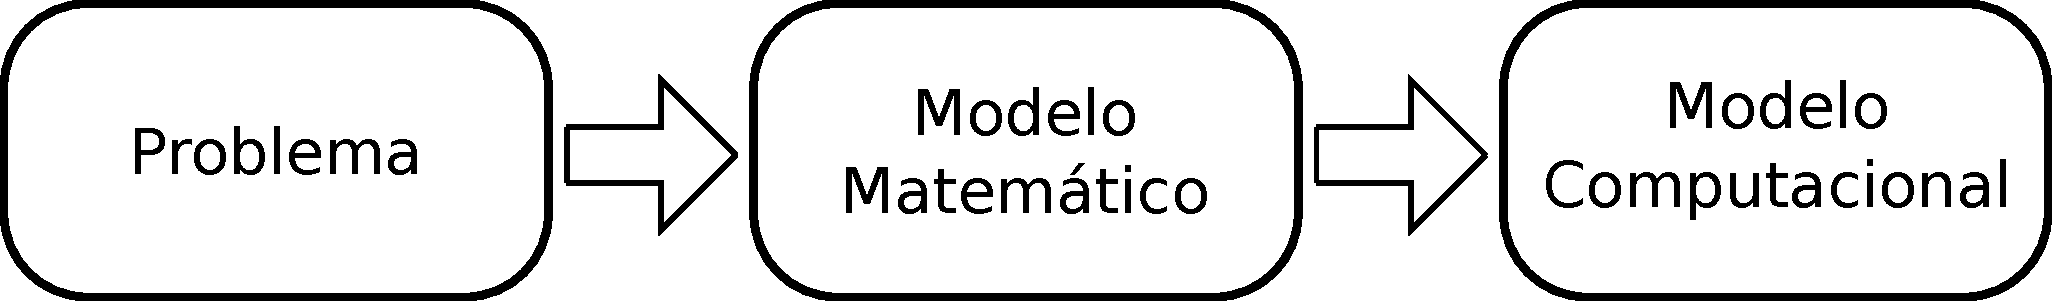
\includegraphics[width=\textwidth]{figs/paradigmas.pdf}
\end{frame}

\begin{frame}{Nosso problema}
    \begin{center}
    Manipular imagens no computador.
    \end{center}
\end{frame}

\begin{frame}{Como vemos uma imagem?}{Luz}
    \begin{figure}
        \centering
        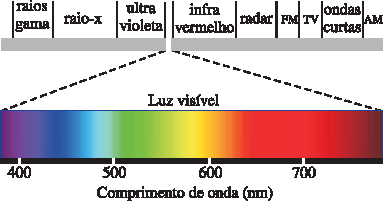
\includegraphics[scale=1.0]{figs/espectro-luz.pdf}
        \caption{Fonte: Gomes, J. e Velho, L., Fundamentos de Computa\c{c}\~ao
        Gr\'afica}
    \end{figure}
\end{frame}

\begin{frame}{Como vemos uma imagem?}{Olho}
    \begin{figure}
        \centering
        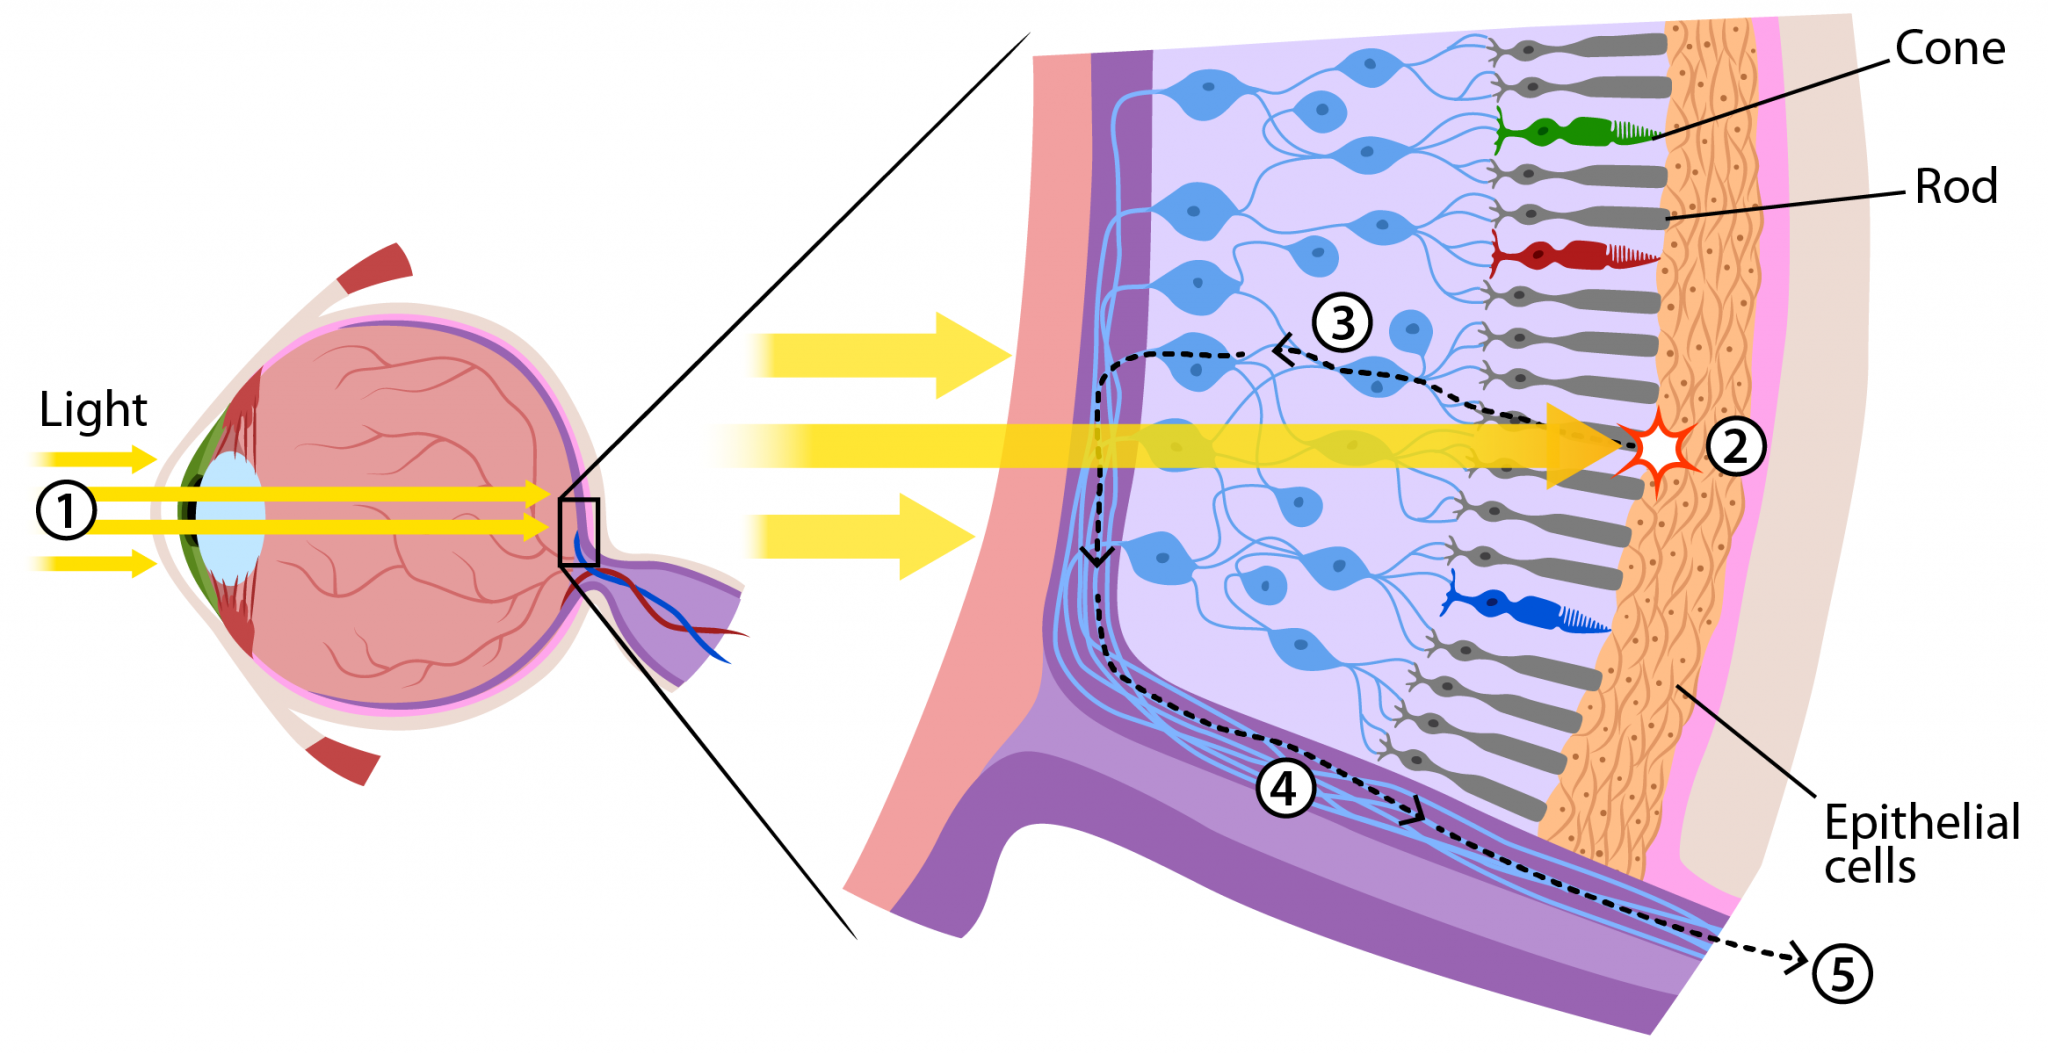
\includegraphics[width=\textwidth]{figs/rods-cones.png}
        \caption{Fonte: https://askabiologist.asu.edu/rods-and-cones}
    \end{figure}
\end{frame}

\begin{frame}{Como vemos uma imagem?}{Sistema {\color{red}R}{\color{green}G}{\color{blue}B}}
    \begin{figure}
        \centering
        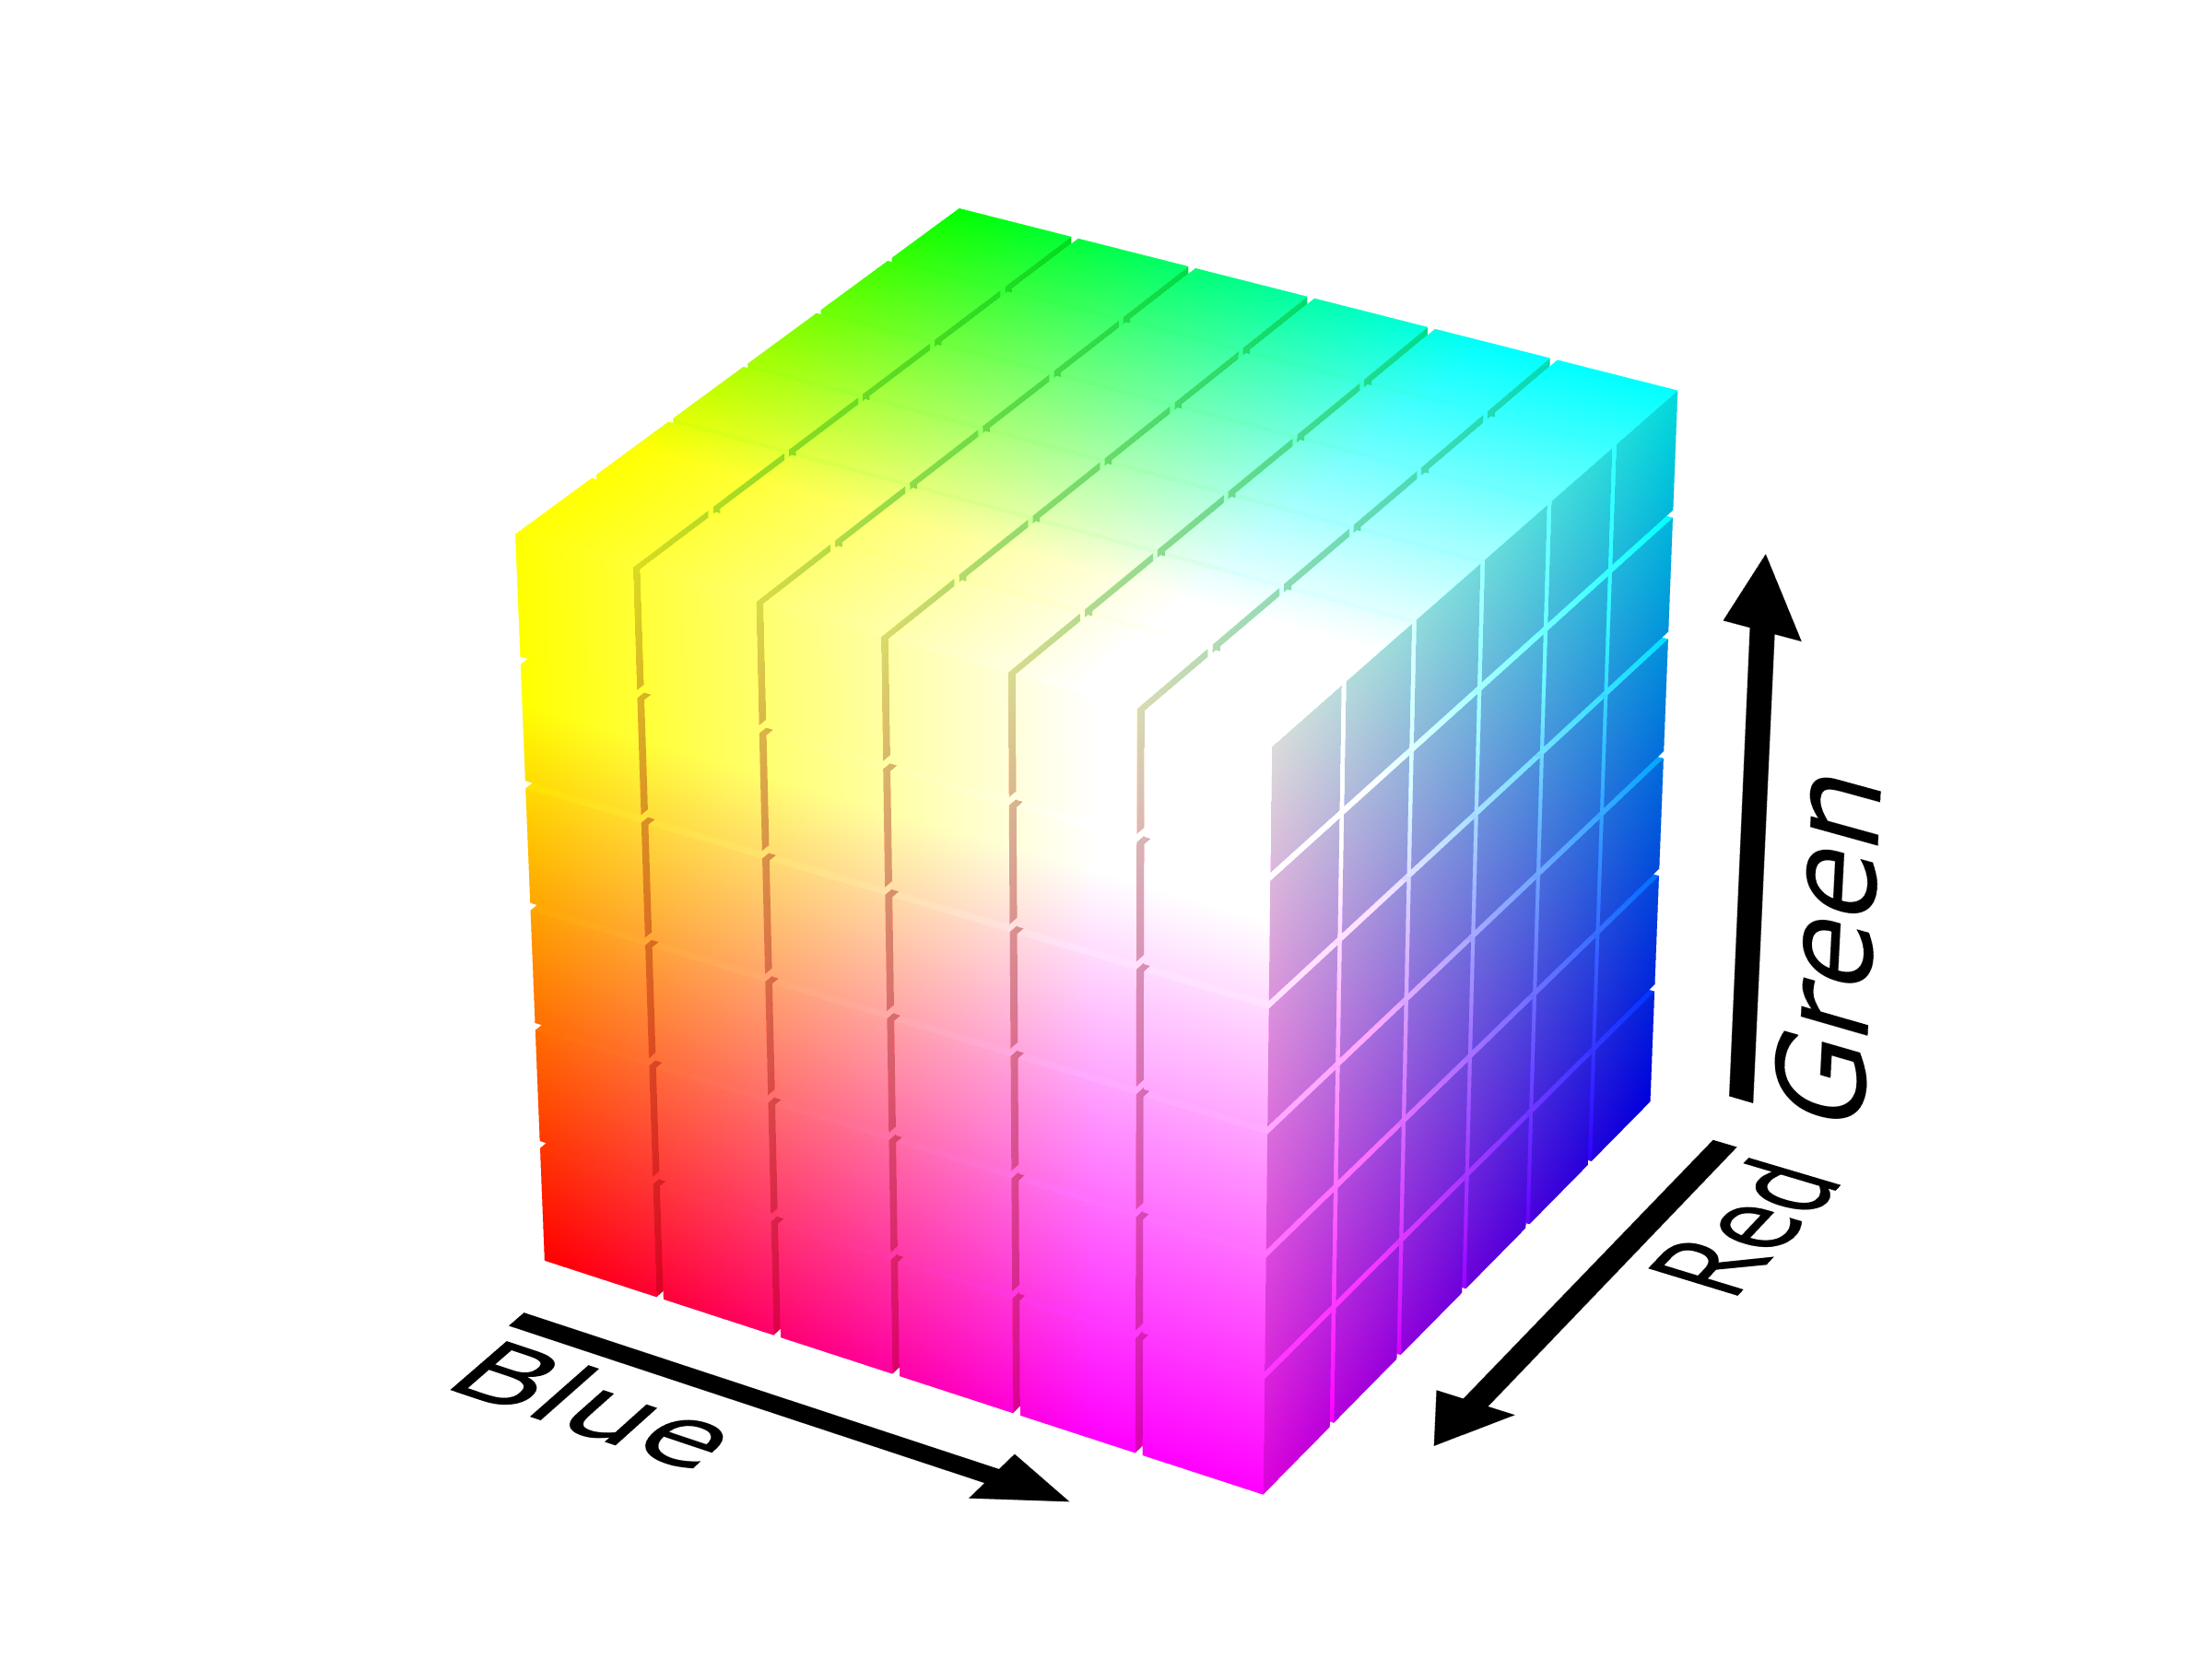
\includegraphics[width=0.8\textwidth]{figs/rgb-cube.png}
        \caption{Fonte: https://en.wikipedia.org/wiki/RGB\_color\_model}
    \end{figure}
\end{frame}

\begin{frame}{Como vemos uma imagem?}{Sistema {\color{red}R}{\color{green}G}{\color{blue}B}}
    \begin{figure}
        \centering
        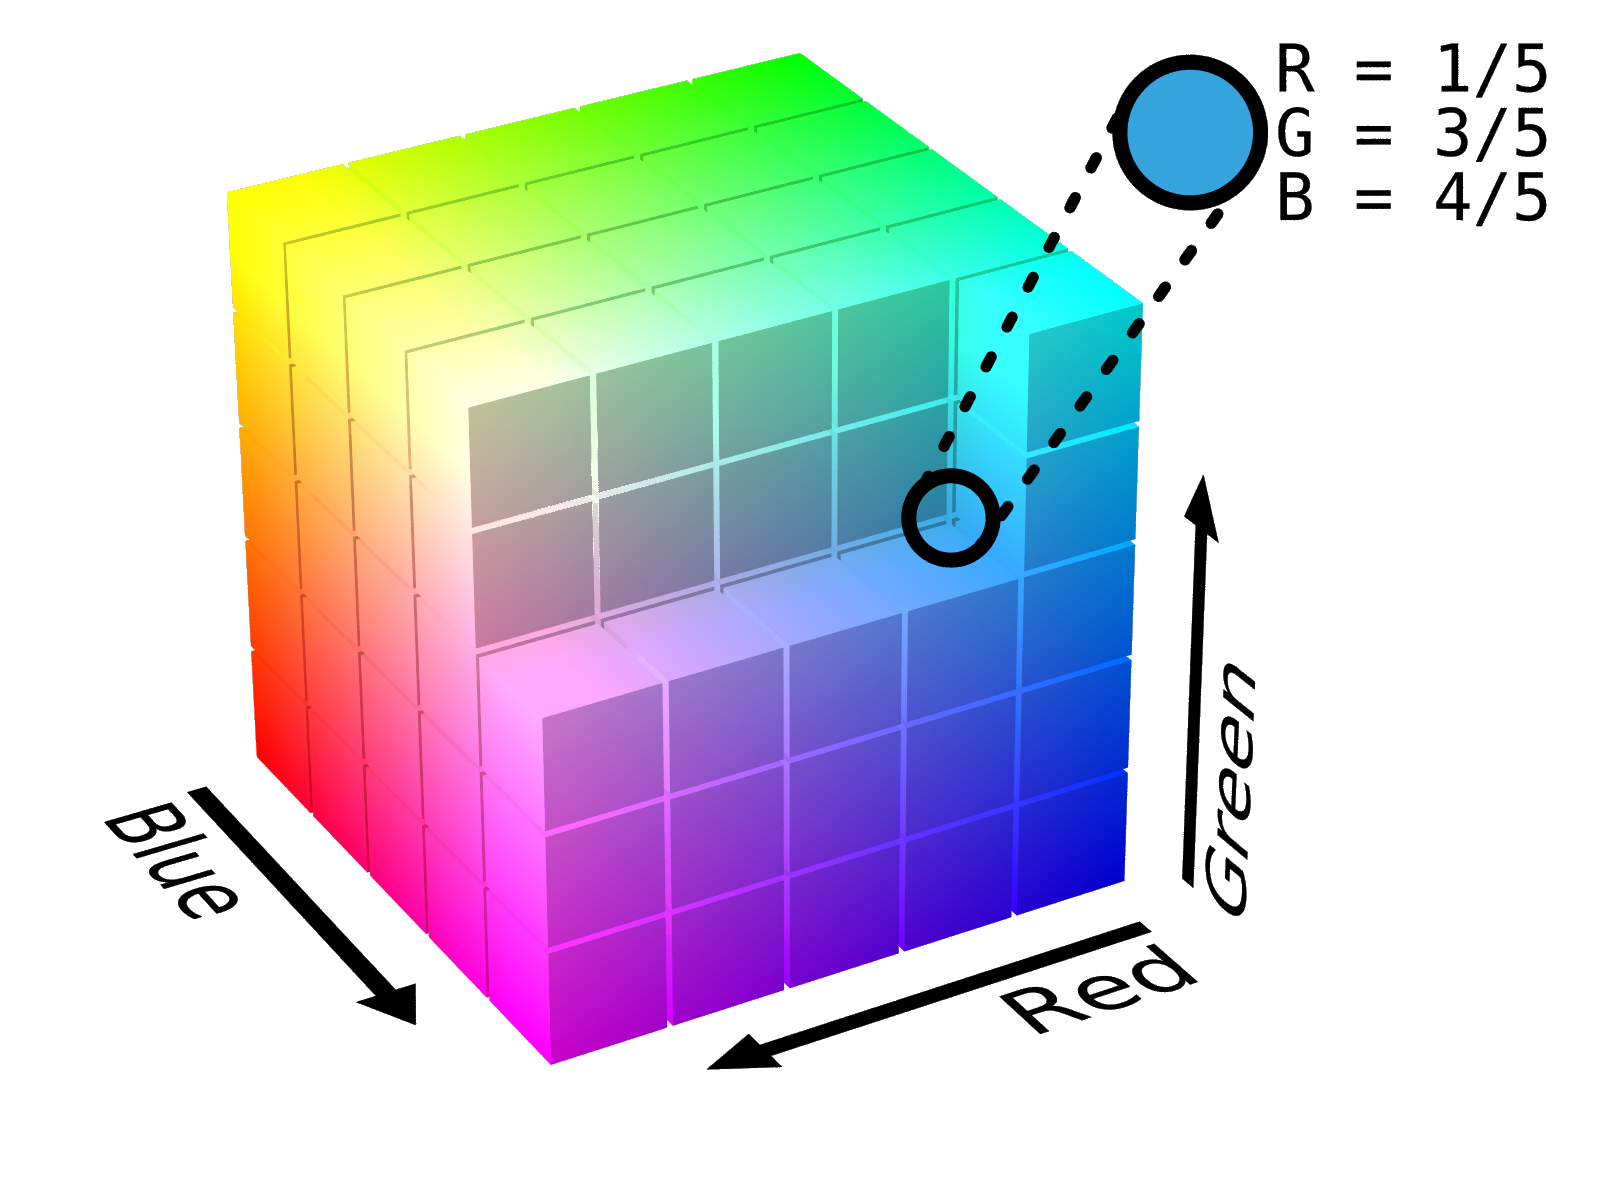
\includegraphics[width=0.8\textwidth]{figs/rgb-point.png}
        \caption{Fonte: https://en.wikipedia.org/wiki/RGB\_color\_space}
    \end{figure}
\end{frame}

\begin{frame}{Uma imagem no computador}
    \begin{figure}
        \centering   
        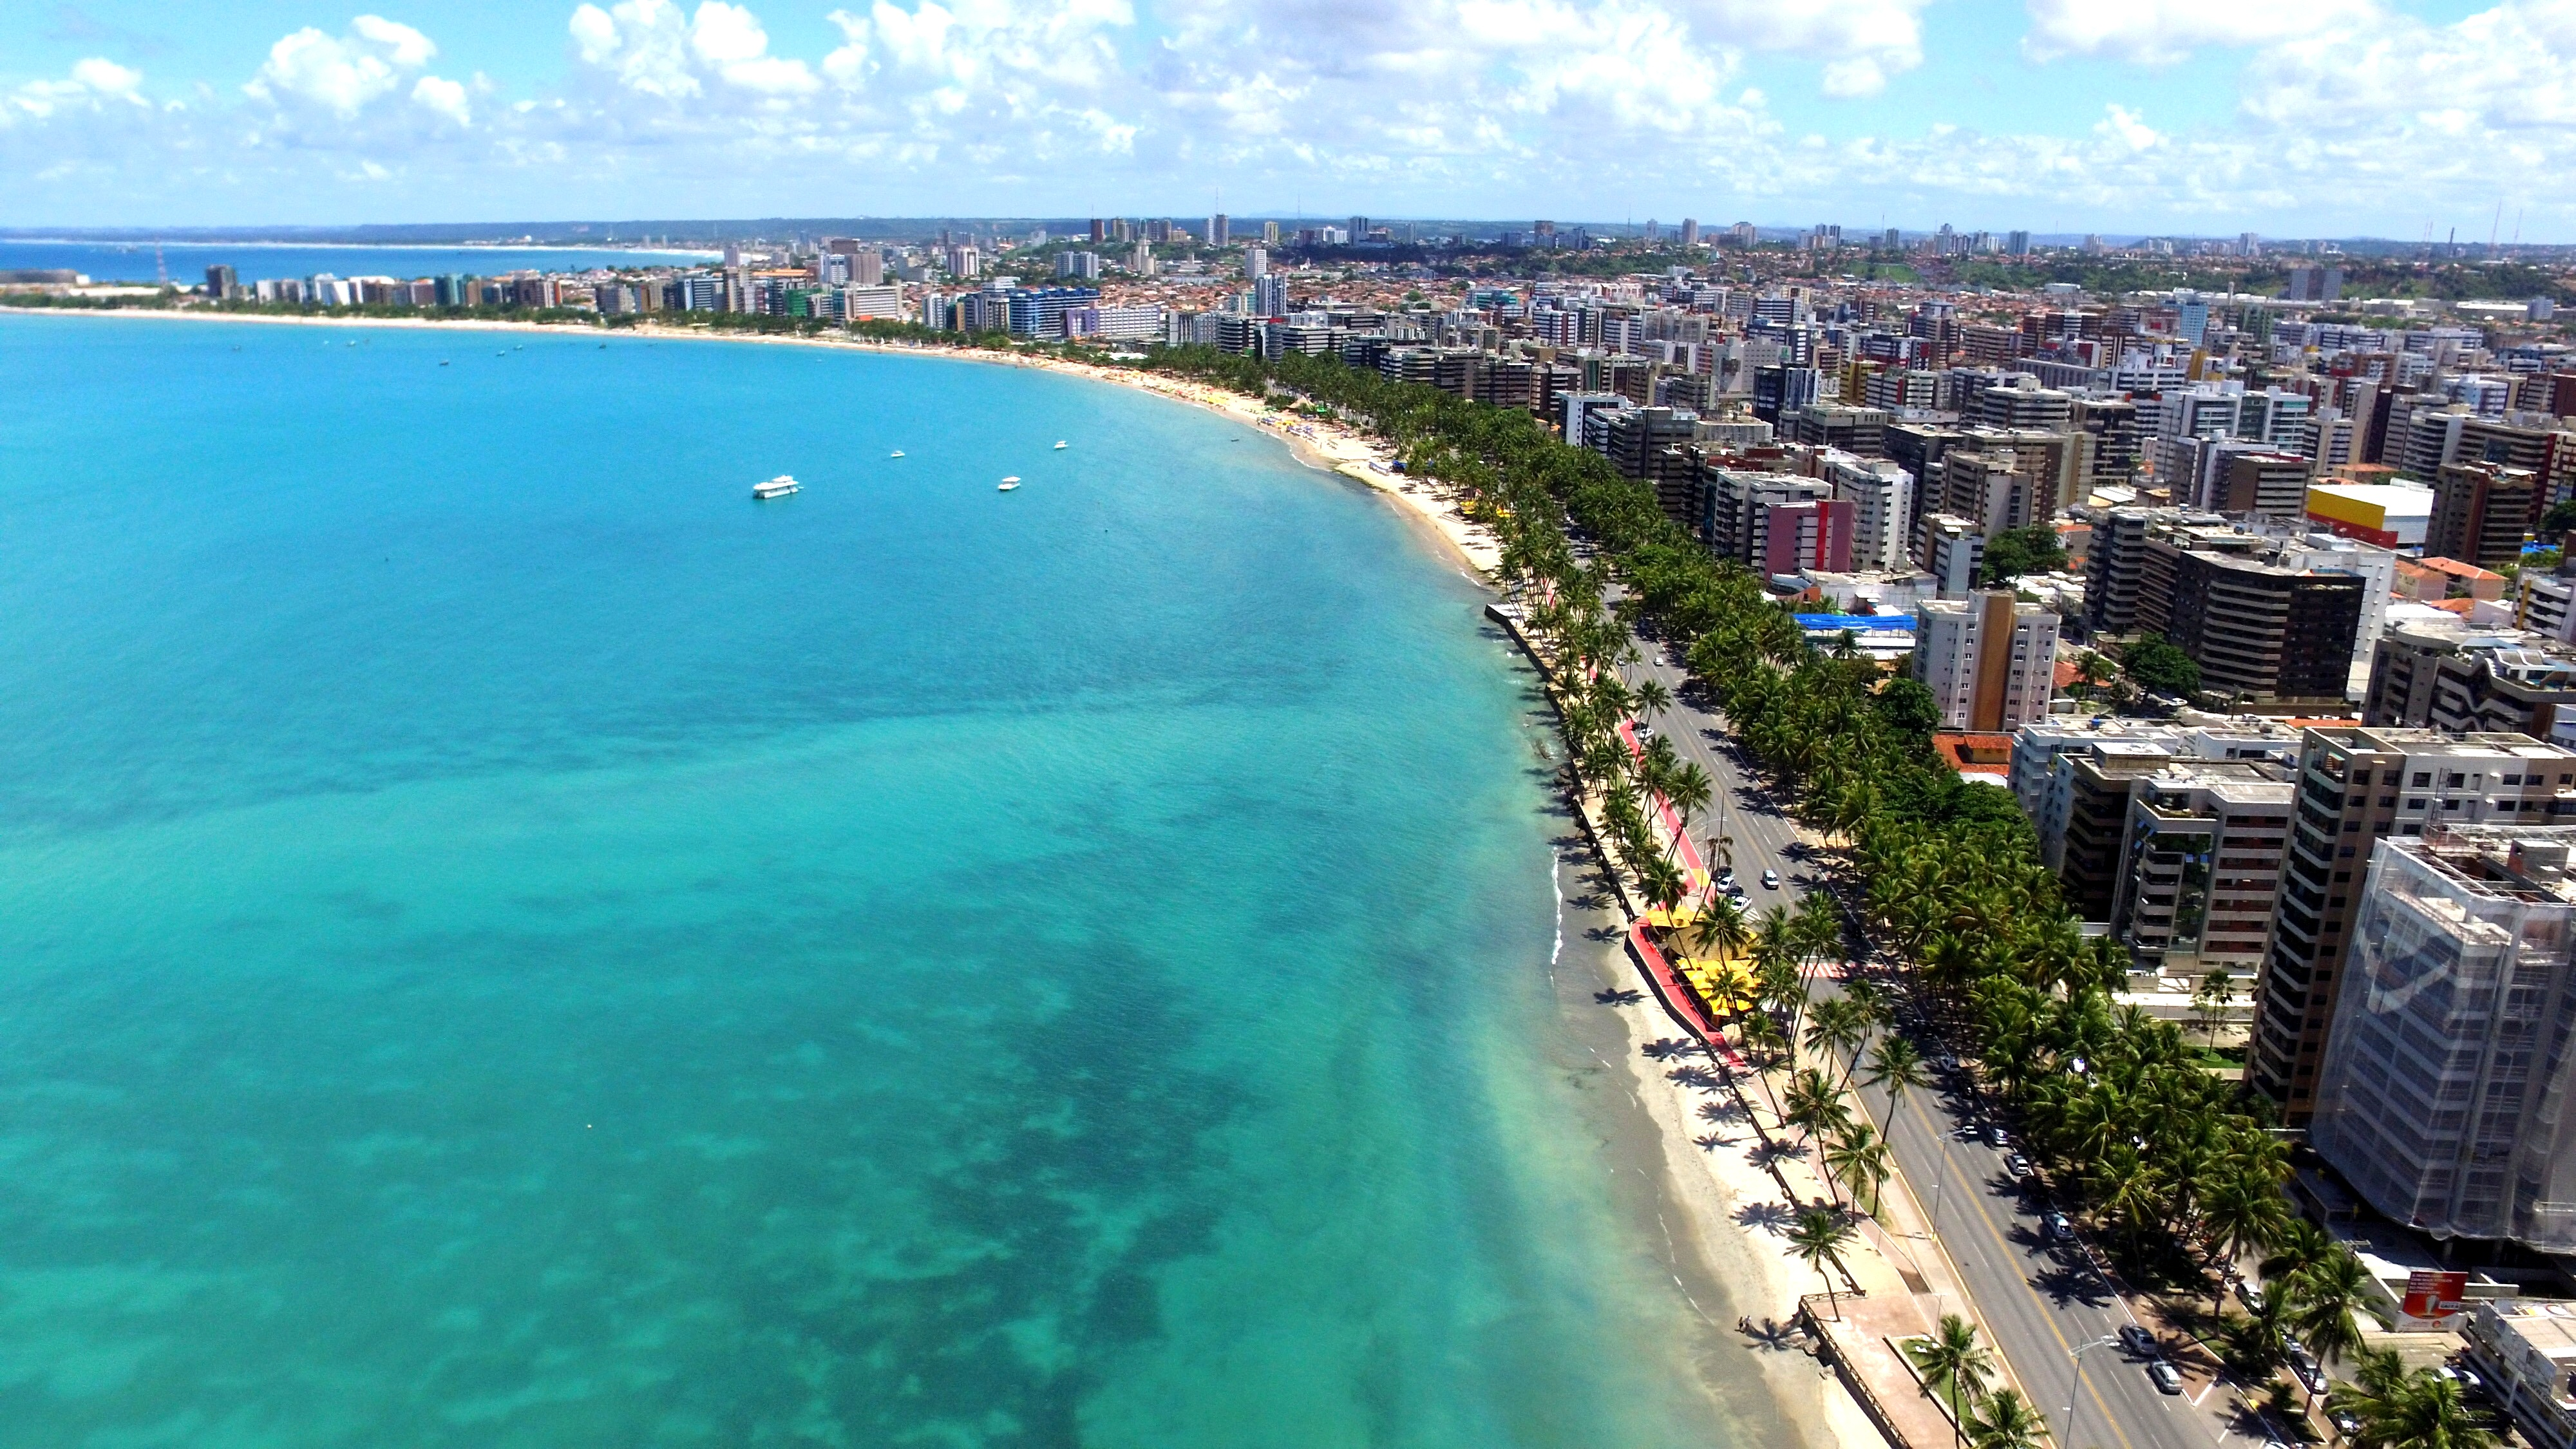
\includegraphics[width=\textwidth]{figs/maceio.jpg}
        \caption{Fonte: M\'arcio no Mundo}
    \end{figure}
\end{frame}

\begin{frame}{Uma imagem no computador}
    \begin{figure}
        \centering   
        \begin{overpic}[width=\textwidth]{figs/maceio.jpg}
            \put(3,3){
\includegraphics[scale=0.15]{figs/maceio-zoom1.png}}  
        \end{overpic}
        \caption{Fonte: M\'arcio no Mundo}
    \end{figure}
\end{frame}

\begin{frame}{Uma imagem no computador}{Matrizes}
    \begin{figure}
        \centering   
        
\includegraphics[scale=0.2]{figs/maceio-zoom2.png}
    \end{figure}
\end{frame}

\begin{frame}{Uma imagem no computador}{Matrizes}
    \begin{figure}
        \centering   
        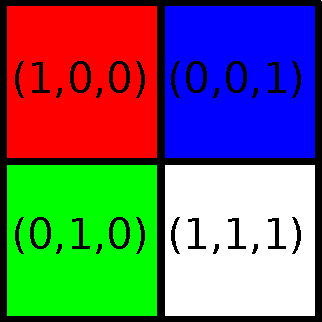
\includegraphics[width=0.5\textwidth]{figs/imagem-matriz.pdf}
    \end{figure}
\end{frame}

\end{document}
